\documentclass[xcolor=dvipsnames]{beamer}
%
% Choose how your presentation looks.
%
% For more themes, color themes and font themes, see:
% http://deic.uab.es/~iblanes/beamer_gallery/index_by_theme.html
%
\mode<presentation>
{
\usetheme{Darmstadt}      % or try Darmstadt, Madrid, Warsaw, ...
\usecolortheme{wolverine} % or try albatross, beaver, crane, ...
\usefonttheme{structurebold}  % or try serif, structurebold, ...
\setbeamertemplate{navigation symbols}{}
\setbeamertemplate{caption}[numbered]
% eigenen stuff definieren
% auf dieser website stehen weiter elemente von denen die farbe geändert werden kann
% http://www.cpt.univ-mrs.fr/~masson/latex/Beamer-appearance-cheat-sheet.pdf
% einfach ausprobieren was passt
\definecolor{Grau}{HTML}{CCCCCC}
\definecolor{GrauDark}{HTML}{777777} % auf weißem hintergrund
\definecolor{Orange}{HTML}{EA5B10}
\setbeamercolor{palette primary}{bg=Grau}
\setbeamercolor{palette primary}{fg=BurntOrange}
\setbeamercolor{normal text}{fg=GrauDark}
\setbeamercolor{structure}{fg=BurntOrange} % farbe der items
\setbeamertemplate{itemize item}[circle]
\setbeamercolor{mini frame}{fg=BurntOrange}
\setbeamercolor{section in head/foot}{bg=Grau}
\setbeamercolor{section in head/foot}{fg=BurntOrange}
\setbeamercolor{subsection in head/foot}{bg=white}
\setbeamercolor{subsection in head/foot}{fg=GrauDark}
\setbeamercolor{headline}{bg=Grau}
\setbeamercolor{block body}{bg=white}
\setbeamercolor{frametitle}{bg=white}

}

\usepackage[utf8]{inputenc}
\usepackage[T1]{fontenc}
\usepackage{ae}
\usepackage{ngerman}
\usepackage{calc}
\usepackage{graphicx}
\usepackage{makecell}
\usepackage{pgfplots}
\usepackage[autostyle=true,german=quotes]{csquotes}
\pgfplotsset{compat=1.4}


\title[Team 2 - Abschlusspräsentation]{CS:Select Abschlusspräsentation - Team 2}
\titlegraphic{\includegraphics[width=\textwidth / 2]{img/logo.png}}
\author{Luca Springer, Alexander Linder, Julian Dinh, Nicholas Bieker,\\ Bendix Sonnenberg}
\date{18.03.2019}

\begin{document}

    \frame[plain]{\titlepage}

    \section{Einleitung}

    \begin{frame}{Problemstellung}
        \center
        \includegraphics[width=\textwidth / 2]{img/logo.png} \\
        \textbf{C}rowd \textbf{S}ourcing: \textbf{Select}
    \end{frame}
    
    \begin{frame}{Feature Subsect Selection - Beispiel: Krebsrisiko}
        \pause
        \begin{columns}
            \begin{column}{0.3\textwidth}
                    \center
                    \onslide<2-> \includegraphics[width=(\textwidth / 3)]{img/teddy.png}
                    \onslide<5-> \includegraphics[width=(\textwidth / 3)]{img/cross.png}
                    \onslide<2-> Hatte Kuscheltiere
            \end{column}
            \begin{column}{0.3\textwidth}
                    \center
                    \onslide<3-> \includegraphics[width=(\textwidth / 4)]{img/cigarette.png}
                    \onslide<5-> \includegraphics[width=(\textwidth / 3)]{img/tick_mark.png}
                    \onslide<3-> \only<3,4>{Raucht}\only<5->{\textbf{Raucht}}
            \end{column}
            \begin{column}{0.3\textwidth}
                    \center
                    \onslide<4-> \includegraphics[width=(\textwidth / 3)]{img/white_shirt.jpg}
                    \onslide<5-> \includegraphics[width=(\textwidth / 3)]{img/cross.png}
                    \onslide<4-> Trägt gerne weiß
            \end{column}
        \end{columns}
        \begin{columns}
            \begin{column}{\textwidth}
                \center
                \onslide<5->\includegraphics[width=(\textwidth / 2)]{img/concerned_doctor.png}
            \end{column}
        \end{columns}
    \end{frame}
    
    \begin{frame}{Gamification}
         \begin{columns}
            \begin{column}{0.5\textwidth}
                \begin{block}{Punkte}
                    \center
                    \includegraphics[width=(\textwidth / 2)]{img/points.png}
                \end{block}
                \begin{block}{Streaks}
                    \center
                    \includegraphics[width=(\textwidth / 2)]{img/streak.png}
                \end{block}
            \end{column}
            \begin{column}{0.5\textwidth}
                \begin{block}{Daily-Challenges}
                    \center
                    \includegraphics[width=(\textwidth / 2)]{img/daily.png}
                \end{block}
            \end{column}
        \end{columns}

    \end{frame}
    \begin{frame}{Gamification}
        \begin{block}{Leaderboard}
        \center
        \includegraphics[width=0.3\textwidth]{img/leaderboard.png}
        \end{block}
        \begin{block}{Achievements}
        \center
        \includegraphics[width=0.3\textwidth]{img/achievment.png}
        \end{block}
    \end{frame}
   \begin{frame}{Spielmodi - Binär-Select}
        \includegraphics[width=\textwidth]{img/binary.png}
    \end{frame}
    \begin{frame}{Spielmodi - Matrix-Select}
        \includegraphics[width=\textwidth]{img/matrix.png}
    \end{frame}
    \begin{frame}{Abgrenzungen}
        Was unser Produkt nicht enthält:
        \begin{itemize}
            \item Machine Learning (Wird extern durchgeführt)
            \item Unterstützung der Auswertung der Daten (Wir sammeln nur mögliche Merkmalsmengen)
        \end{itemize}
    \end{frame}
 
    \renewcommand{\arraystretch}{1.5}

	\section{Softwaretechnik}
	\begin{frame}{Grundaufbau}
	\centering
	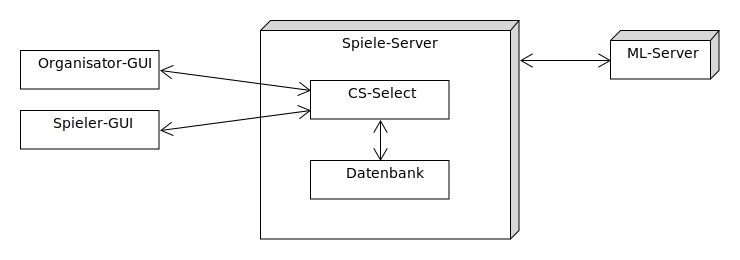
\includegraphics[width=\textwidth]{img/Architektur.pdf}
	\end{frame}

	\begin{frame}{Paketdiagramm}
	\centering
	\includegraphics[width=\textwidth]{img/Klassendiagramm.png}
	\end{frame}
	
    \section{Statistiken}
    
    \begin{frame}{Unit-Tests}
    \centering
    \begin{tikzpicture}
    \begin{axis}[
    ybar,
    enlarge x limits=0.2,
    width=0.95\textwidth,
    height=0.8\textheight,
    ylabel={Anzahl},
    xtick=data,
    nodes near coords,
    ymin=0,
    legend pos=north west,
    xticklabel style={rotate=45},
    symbolic x coords={User,Database,Game,Gamification,Configuration},xticklabels={User,Database,Game,Gamification,
    Configuration},
    ]
    
    \addplot coordinates
    {(User,17) (Database,64) (Game,74) (Gamification,36) (Configuration,16)};
    \end{axis}
    \end{tikzpicture}
    Insgesamt 215 Testcases
\end{frame}

    \begin{frame}{Testüberdeckung}
        \centering
        \begin{tikzpicture}
            \begin{axis}[
            ybar,
            enlarge x limits=0.2,
            width=0.95\textwidth,
            height=0.8\textheight,
            ylabel={Prozent},
            xtick=data,
            nodes near coords,
            ymin=0,
            legend pos=north west,
            xticklabel style={rotate=45},
            symbolic x coords={User,Database,Game,Gamification,Configuration},xticklabels={User,Database,Game,Gamification,Configuration
            },
            ]

                \addplot coordinates
                {(User,37) (Database,79) (Game,89) (Gamification,92) (Configuration,100)};
            \end{axis}
        \end{tikzpicture}
        Insgesamt 81 Prozent
    \end{frame}

	\begin{frame}{Lines of Code}
	\centering
	\includegraphics[width=\textwidth]{img/Codezeilen.png}
	\end{frame}
	
    \begin{frame}{Lines of Code}
        \begin{table}[t]
            \begin{center}
                \begin{tabular}{ | l | c | }
                    \hline
                    Datei & Anzahl Zeilen \\
                    \hline
                    Java & 8218 \\
                    JavaScript & 1866 \\
                    JavaServer Pages & 491 \\
                    XML & 331 \\
                    Properties & 493 \\
                    CSS & 100 \\ \Xhline{0.8pt}
                    Gesamt (inklusive Kommentar- und Leerzeilen) & 16682 \\ \hline
                \end{tabular}
            \end{center}
        \end{table}
    \end{frame}


    \begin{frame}{GitHub - CS:Select}
        \centering
        \begin{tikzpicture}
        \begin{axis}[
        ybar,
        enlarge x limits=0.2,
        width=0.95\textwidth,
        height=0.8\textheight,
        ylabel={Anzahl Commits pro Woche},
        xtick=data,
        nodes near coords,
        ymin=0,
        legend pos=north west,
        xticklabel style={rotate=45},
        symbolic x coords={6.1.,13.1.,20.1.,27.1.,3.2.,10.2.,17.2.,24.2.,3.3.},xticklabels={6.1.,13.1.,20.1.,27.1.,3.2.,10.2.,17.2.,24.2.,3.3.
        },
        ]
        
        \addplot coordinates
        {(6.1.,55) (13.1.,134) (20.1.,165) (27.1.,181) (3.2.,84) (10.2.,162) (17.2.,25) (24.2.,35) (3.3.,99)};
        \end{axis}
        \end{tikzpicture}
        Insgesamt 1008 Commits, 168 Issues closed
    \end{frame}

    \section{Tools}
    \begin{frame}{Allgemein}
        \begin{columns}
            \begin{column}{0.3\textwidth}
                \begin{block}{UML}
                    \center
                    \includegraphics[width=(\textwidth / 2)]{img/vispar.png} %TODO find better logo
                \end{block}
            \end{column}
            \begin{column}{0.3\textwidth}
                \begin{block}{Unit-Testing}
                    \center
                    \includegraphics[width=(\textwidth / 3)]{img/junit.png}
                \end{block}
                \begin{block}{IDE}
                    \center
                    \includegraphics[width=\textwidth / 4]{img/intellij.pdf}
                \end{block}
            \end{column}
                \begin{column}{0.3\textwidth}
                    \begin{block}{Continuous Integration}
                        \includegraphics[width=(\textwidth)]{img/travis.png}
                    \end{block}
                    \begin{block}{Statische Codeanalyse}
                        \center
                        \includegraphics[width=(\textwidth / 4)]{img/codacy.pdf}
                        Codacy\\
                        \includegraphics[width=(\textwidth / 2)]{img/checkstyle.png}
                    \end{block}
                \end{column}
        \end{columns}
    \end{frame}

    \section{Lernerfahrung}
    \begin{frame}
        \begin{center}
            \only<1>{\Huge Was haben wir gelernt?}
            \only<2> \includegraphics[width=(\textwidth/2)]{img/javascript.png}
        \end{center}
    \end{frame}

    \appendix
    \begin{frame}[plain]
        \begin{itemize}
            \item https://www.clker.com/clipart-26656.html \\
            \item https://www.skillscommons.org/handle/taaccct/8679 \\
            \item https://en.wikipedia.org/wiki/File:Red\_x\_large.png \\
            \item https://art4clip.com/explore/Brown\%Bear\%clipart\%brown\%objects/ \\
            \item https://www.istockphoto.com/de/grafiken/button-up-shirt-template-cartoon \\
            \item https://wildlifehexagon.wordpress.com/2016/06/19/binging-on-free-code-camp-algorithm-challenges-aka-bonfires/ \\
            \item https://commons.wikimedia.org/wiki/File:Check-green.svg \\
        \end{itemize}
    \end{frame}
\end{document}
